 

\documentclass{article}
\usepackage{float}
\usepackage{amsmath,amssymb,amsthm,graphicx}
\usepackage{subcaption}
\usepackage{mleftright}
\usepackage{tikz}
\usepackage{tikz-network}


\setlength{\oddsidemargin}{0.25 in}
\setlength{\evensidemargin}{-0.25 in}
\setlength{\topmargin}{-0.6 in}
\setlength{\textwidth}{6.5 in}
\setlength{\textheight}{8.5 in}
\setlength{\headsep}{0.75 in}
\setlength{\parindent}{0 in}
\setlength{\parskip}{0.1 in}

\newtheorem{theorem}{Theorem}
\newtheorem{corollary}{Corollary}
\newtheorem{proposition}{Proposition}
\newtheorem*{remark}{Remark}
\theoremstyle{definition}
\newtheorem{example}{Example}
\newtheorem{definition}{Definition}

\newcommand{\lecture}[4]{
   \pagestyle{myheadings}
   \thispagestyle{plain}
   \newpage
%   \setcounter{lecnum}{#1}
   \setcounter{page}{1}
   \noindent
   \begin{center}
   \framebox{
      \vbox{\vspace{2mm}
    \hbox to 6.58in { {\bf CSC~565: Graph Theory
                        \hfill North Carolina State University} }
    \hbox to 6.58in { {\bf Fall 2019
                        \hfill Computer Science} }
       \vspace{4mm}
       \hbox to 6.28in { {\Large \hfill Lecture #1: #2  \hfill} }
       \vspace{2mm}
       \hbox to 6.28in { {\it Lecturer: {\it Don Sheehy {\tt <drsheehy@ncsu.edu>}} \hfill Scribe: #4} }
      \vspace{2mm}}
   }
   \end{center}
   \markboth{Lecture #1: #2}{Lecture #1: #2}
   \vspace*{4mm}
}


\begin{document}
    \lecture{26}{Nov 20, 2019}{}{Niranj Jyothish, Xun Jia}
    
    \section{Overview}
    In the previous lectures we have talked about the algebra in graph theory. We turn a graph into a matrix, we build vector space in approach of vertices, edges, we introduce the definition of kernel, adjaceny matrix, incidence matrix, etc.Today we are going to try to solve linear equations in a perspective of graph.
    
    \section{Preview}
    We have already learned how to solve linear equation systems by gaussian elimination and back substitution. But the cost can be super big. In this lecture we first show the complexity of gaussian elimination, then we show the graph approach and vertex elimination. Also we will talk about the order of vertex elimination which can keep the vertex sparse and shows how to find it with a grid as an example. Finally, we talk a little bit of separator associated theorems.
    
    
    \section{Gaussian elimination and vertex elimination}
    Gaussian elimination is a classic method to solve linear systems. But the problem is that it has a high cost in both time and space. We will show the complexity of gaussian elimination and then introduce vertex elimination.
    
    Suppose we have a matrix $A$ and a system $Ax=b$, in gaussian elimination, we try to operate the matrix like:
    \[
    LA = U
    \]
    where L is lower triangular and U is upper triangular, Let's take the first step of this process as an example.
    The first step can be described as following:
    $$ A \longrightarrow \begin{bmatrix}
    \star & \cdots & \cdots & \cdots \\
    0 & \cdots & \cdots & \cdots \\
    0 & \cdots & \cdots & \cdots \\
    0 & \cdots & \cdots & \cdots \\
    \end{bmatrix} $$\newline
    For each element in the first column, we need to calculate the coefficients and do the addition, which has a  cost of $Olog(n^2)$. For the whole matrix, the complexity will be:
    \[
    \sum_{i=1}^nO(n^2) = O(n^3)
    \]
    If the matrix is sparse, which means there are only constant numbers of non-zero elements in a row, we could do this in a constant time. But there is a problem: The matrix is not always sparse. It's not garunteed that we end up with sparse matrix. So keeping the graph sparse is critical. How to keep the matrix sparse? Here comes the graphs.
    
    
    If A is n$\times$nsymmetric, we can do the same operations on rows and columns by left-multipy L and right-multiply $L^T$. For example, we eliminate the rows and columns like this: 
    $$ \begin{bmatrix}
    1 & 2 & 3 \\
    2 & \cdots & \cdots  \\
    3 & \cdots & \cdots  \\
    \end{bmatrix}
    \longrightarrow
    \begin{bmatrix}
    1 & 0 & 0 \\
    0 & \cdots & \cdots  \\
    0 & \cdots & \cdots  \\
    \end{bmatrix}
     $$
     Now we can associate a graph to represent the matrix, in other word, a linear system. The representation is:
     \[
     Graph(A)=(\{1, \cdots, n\},\{(i, j):A_{ij}\neq0, i \neq j \})
     \]
     Note that the graph doesn't capture all the information of the matrix. Many matrices give the same graph. We don't expect just look at the graph and know the solution the equation system. It only gives us a summary that where the non-zero elements are.
    Now if we do one steps, or let's say removing one variable in the system, we can regard now as removing a vertex from a graph. But new edges come from removing. So the question now is which new edge appears? The point is that if we now the graph always stays sparse, we know that the matrix always stays sparse, and then we can give a solid upper bound of the complexity. Now let's see which new edges can appear in a graph.
    $$A = \begin{bmatrix}
    3 & -1 & -1 & -1 \\
    -1 & 1 & 0 & 0 \\
    -1 & 0 & 1 & 0 \\
    -1 & 0 & 0 & 1 \\
    \end{bmatrix}$$
    \begin{figure}[h!]
    	\begin{center}
    		\begin{tikzpicture}
    		\Vertex[x=1,y=1, label = 1] {1}
    		\Vertex[x=1,y=2.44, label = 2] {2}
    		\Vertex[x=2,y=0, label = 3] {3}
    		\Vertex[x=0,y=0, label = 4] {4}
    		
    		\Edge[color = black, lw = 2pt](1)(2)
    		\Edge(1)(3)
    		\Edge(1)(4)
    		
    		\end{tikzpicture}
    	\end{center}
    	\caption{Graph Laplacian of G}
    \end{figure}
	Given a matrix A, eliminating the first variable and get:
	$$LA =
	\begin{bmatrix}
	1 & 0 & 0 & 0 \\
	\frac{1}{3} & 1 & 0 & 0 \\
	\frac{1}{3} & 0 & 1 & 0 \\
	\frac{1}{3} & 0 & 0 & 1 \\
	\end{bmatrix}
	\begin{bmatrix}
	3 & -1 & -1 & -1 \\
	0& 1 & 0 & 0 \\
	0 & 0 & 1 & 0 \\
	0 & 0 & 0 & 1 \\
	\end{bmatrix}
	=
	\begin{bmatrix}
	3 & -1 & -1 & -1 \\
	-1 & \frac{2}{3} & -\frac{1}{3} & -\frac{1}{3} \\
	-1 & -\frac{1}{3} & \frac{2}{3}& -\frac{1}{3} \\
	-1 & -\frac{1}{3} & -\frac{1}{3} & \frac{2}{3} \\
	\end{bmatrix}
	$$
	Eliminate the row by right-multiply $L^T$ and get:
	$$LAL^T = \begin{bmatrix}
	3 & 0 & 0 & 0 \\
	0 & \cdots & \cdots & \cdots \\
	0 & \cdots & \cdots & \cdots \\
	0 & \cdots & \cdots & \cdots \\
	\end{bmatrix}$$
	We can see the new matrix can be super dense, even it is sparse in the previous step. 
	
	Take $LA_{23}$ as an example, it turns into non-zero because there is an edge between $v_1$ and $v_2$ and between $v_1$ and $v)3$. Generealy speaking, there is a fill edge only if we have two vertices both adjacent to the vertex we are removing.
	
	Figure 2 shows the graph after removing a vertex according to the matrix operations.
	
    \begin{figure}[h!]
    	\begin{center}
    		\begin{tikzpicture}
    		\Vertex[x=1,y=1, label = 1] {1}
    		\Vertex[x=1,y=2.44, label = 2] {2}
    		\Vertex[x=2,y=0, label = 3] {3}
    		\Vertex[x=0,y=0, label = 4] {4}
    		
    		\Edge[color = black, lw = 2pt](4)(2)
    		\Edge(2)(3)
    		\Edge(3)(4)
    		
    		\end{tikzpicture}
    	\end{center}
    	\caption{Graph G after removing a vertex}
    \end{figure}
    
    Now we can associate vertex elimination with vertex elimination:
    \textbf{Removing a vertex v adds a clique on neighbors of v}.
    
    
    Tiny change in the oder of removing vertices makes huge difference. Consider a star gparh with n vertices. Removing the center vertex leads to $K_{n-1}$ while removing a leaf keeps it a star graph, which means the graph is still sparse. That means the order of vertices removing is critical. With a good order, we can eliminate the graph as well as keep the graph sparse, in other words, keep the matrix sparse. The following will talk about the order.
    
    \section{Nested Dissection and order finding}
    Finding an optimal order can be very hard which is an NP-hard problem. Let's take a grid as an example.
    \begin{figure}[h!]
    	\begin{center}
    		\begin{tikzpicture} 
    		\draw[help lines] ( 0,0 ) grid ( 4, 4); 
    		\draw[red] (2,0) -- (2,4); 
    		\draw[red] (0,2) -- (4,2); 
    		\end{tikzpicture}
    	\end{center}
    	\caption{Grid with a separator}
    \end{figure}
	\begin{definition}
		A vertex separator is a subset S $\in$ V such that G$\backslash$S is disconnected.
	\end{definition}
	Finding a separator means we will elinimate it at last. Besides, we also want the separator gives us roughly equal-sized pieces. In the concept of divide and conquer, the success to make parts equal garanteed a $O(logn)$ complexity. However, if it is not, we may end up with more work. So the goal is to find small separators with roughly equal-sized pieces.
	\begin{definition}
		Nested dissection: Finding a separator and recursively finding separators in the pieces we get from the current separator.
	\end{definition}
	Take a separator tree of a grid as an example:
	
	\begin{figure}[h!]
		\begin{center}
			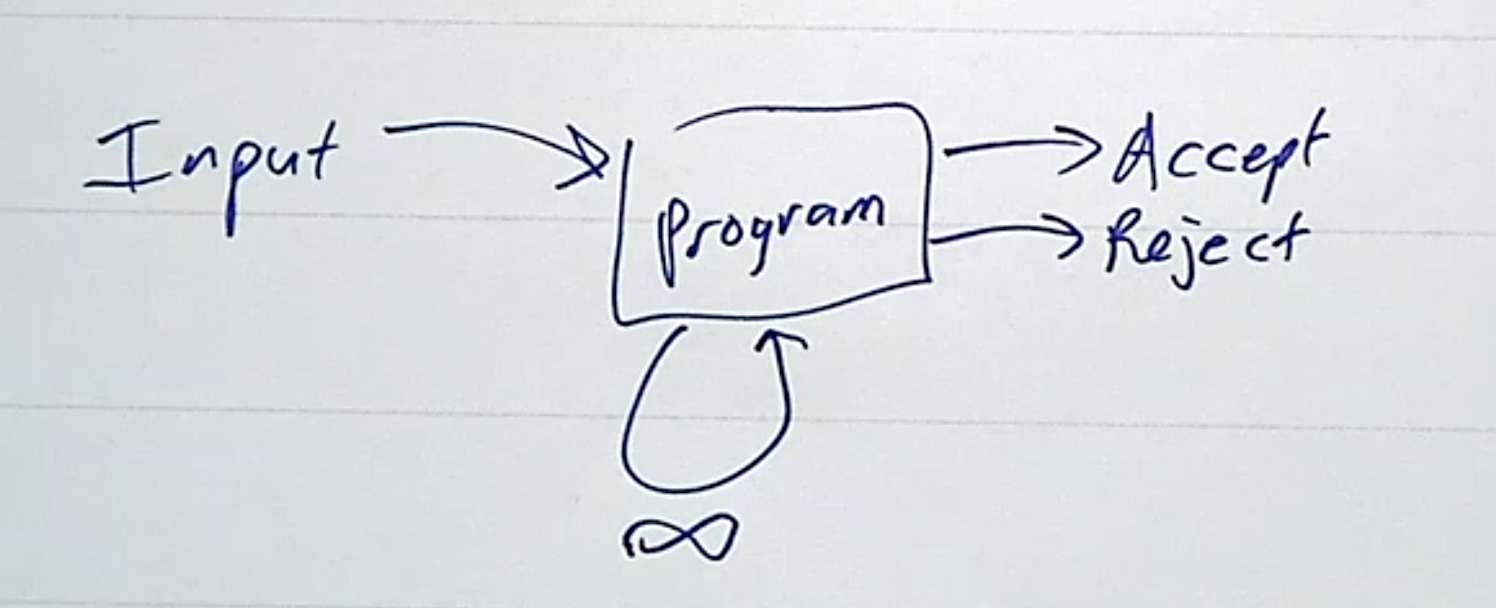
\includegraphics[scale=0.3]{fig1}
		\end{center}
		\caption{Separator tree}
	\end{figure}

	By building a separator tree, we can build an elimination order by elinimating the tree from bottom up. Actually, \textbf{Recursively find separators order the vertices bottom up. } 
	
	In the case of grid graph, consider that if we don't do the nested dissection, removing the first row will lead to fill edges appear between each pair of vertices in the second row, which end up with a very dense graph.
	
	The reasoning of where fill edge can appear is that if we eliminate everything in a path (u,v), we will get a fill edge from u to v. In fact, \textbf{there will be a fill edge (u,v) if there is a path u,v such that evey interior vertex is eliminated before u,v. }
	\begin{figure}[h!]
		\begin{center}
			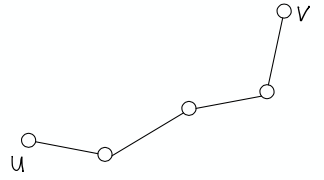
\includegraphics[scale=0.3]{fig2}
		\end{center}
		\caption{Fill edge in a path}
	\end{figure}
    
    Go back to the grid graph, now we will see how many fill edges we will get if we do the nested dissection. 
    
    \begin{figure}[h!]
    	\begin{center}
    		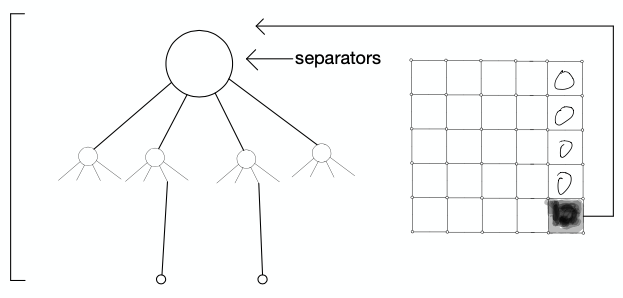
\includegraphics[scale=0.3]{fig3}
    	\end{center}
    	\caption{Separator tree}
    \end{figure}
	
	Note that there will not be a fill edge between different level vertices. 
	
	Since the depth of the tree is log(n), what we should do now is to count the fill edges for each level in the tree. If there is a path from a vertex to a higher level separator which only goes through the vertex elinimated before, there will be a fill edge from it to the higher level separator, so for a n$\times$n grid, we get totally
	\[
	f(n) = 2\sqrt{n}(\frac{n}{4}) + 4f(\frac{n}{4})
	\]
	fill edges.
   This recursion can be really bad, which is not much better than naive order. But not all parts of the pieces can have access to the higher level separator. That means we will lose a whole bunch of vertices even go one step deeper to the tree.
   
   Let's jump to the conclusion that the number of  fill edges to the top level separator is
   \[
   f(n) = 24n + 4f(\frac{n}{4})
   \]
   
   In fact, we have theorems for all the graphs other than grid graph.
   \begin{theorem}
   	[Planar Separator Graph]
   	Every planar graph has a O($\sqrt{n}$) size separator that divides it into components of size $\leq$ $\frac{3n}{4}$.
   \end{theorem}
	\begin{theorem}
		Planar graph can be "eliminated" with O(nlogn) fill and O($n^{\frac{3}{2}}$) mathematical operations.
	\end{theorem}


   
\end{document}
